\begin{figure}[htb!]
    \centering
    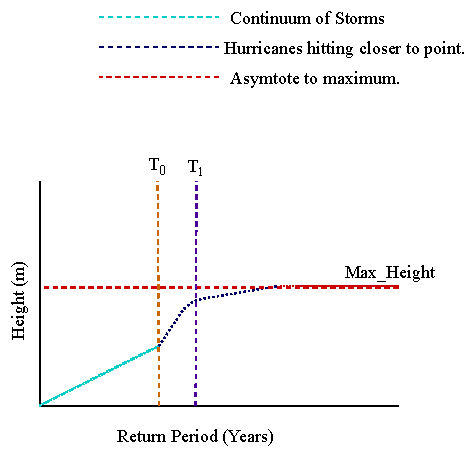
\includegraphics[width=1\linewidth]{images/Return_Hypothesis.pdf}
    \vspace{-15pt}
   \caption{The maximum height is a function of the potential intensity
   allowed by the climate, and the responsiveness of that point on the coastline to a
   wind stress of that size. If T$_0$ is a similar or greater than the time period of
   measurement, then it is possible that no hurricanes exist in the data sample.
   Absence of evidence is not evidence of absence however, and some areas of the US
   coastline such as Galverston and New England experience hurricanes infrequently,
   but as respectively in 1900 and 1908, when they do come they can cause great devastation~\cite{emanuel2005divine}.
   The low TC frequency bias in CMIP models will exacerbate this problem. This will
   appear as the blue curve continued upwards. The period of time
   between T$_0$ and T$_1$ likely depends on the average size of the tropical cyclone storms, and the
   percentage of them which rise to their maximum severity.
   For highly irresponsive places (e.g. Miami), it is possible that the deviation caused
   by hurricane landfall does not cause a large deviation from the existing EV distribution,
   that is mainly caused by other factors (the Florida current).
   }
   \label{fig:return_hyp}

\end{figure}
